\documentclass{article}
\usepackage{graphicx} % Required for inserting images
\usepackage{amsmath}
\usepackage[english, russian] {babel}
\usepackage[utf8]{inputenc}
\usepackage[T2A]{fontenc}
\usepackage{minted}
\usepackage{float}
\usepackage{amssymb}
\usepackage{mathtools}

\title{Дефференцальные уравнения. Лекции}
\author{silvia.lesnaia }
\date{February 2025}

\begin{document}

\maketitle

\textbf{14.02.25}

\section{Литература}
1. В.В Степанов. Курс дифференциальных уравнений (вообще можно любые учебники использовать)
2. А.Ф Филипов Сборник задач дифференциальных уравнений 

\section{ВВЕДЕНИЕ}

ОПР: Обыкновенные дифференциальные уравнения n-го порядка имеет вид F(x,y,y',.. y$^(n)$)=0 где x независимая переменная, y'=y'(x),... y\^(n)=y$^n$(x),

$F=F(t_1,t_2,..,t_n) Функция \varphi (x) называется решением (частичным) уравнения 1 если  F (x, \varphi(x), \varphi'(x),..., \varphi^n (x)  \equiv 0 $


Законы природы написаны на языке дифференциальных уравнении - Ньютон

Примеры:

1. Уравнение радиоактивного распада

x - время, y(x) - количество рад. вещества в момент времени x

\begin{figure}[H]
    \centering
    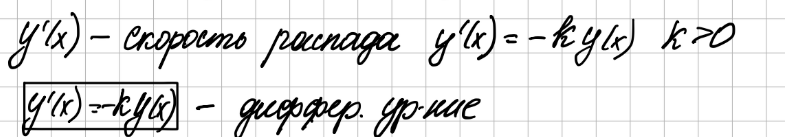
\includegraphics[width=0.5\linewidth]{Снимок экрана 2025-02-14 101634.png}
\end{figure}

2. Уравнение малых колебаний маятника

x - время y(x)- угол отклонения от положения равен 2??

y''+ $\frac{g}{l}$ *y(x)=0

\begin{figure}[H]
    \centering
    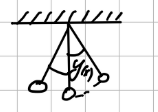
\includegraphics[width=0.3\linewidth]{Снимок экрана 2025-02-14 102205.png}
\end{figure}

\section{Дифференциальные уравнения первого порядка}

ОПР: Деф.урав.1го порядка это уравнения вида F(x,y,y') = 0 или y'=f(x,y) (нормальная форма)

ОПР: Деф.урав.1го порядка в симметричной форме имеет вид A(x,y),  B(x,y) = 0, где A(x,y),  B(x,y) - заданные функциями.

Если y=y(x), то(2) $\iff$  $\frac{dy}{dx}$ = +$\frac{A(x,y)}{B(x,y)}$ (3)

Если x=x(y), то(2) $\iff$  $\frac{dy}{dx}$ = -$\frac{A(x,y)}{B(x,y)}$(3)

Можно показать


\subsection{Дифференциальные уравнения с разделяющимися переменным}

Уравнение с разделяющимися переменными имеет вид:

y'=f(x,y) - общий вид

y'=x+y такое не распадется - частный случай

Алгоритм решения:

 1. Переходим к дифференциалу 
 
    $\frac{dy}{dx}$ = $f_1$(x) $f_2$(y) | *dx, $\frac{1}{ f_2 (y)}$ 

 2. Делим переменные (Разделение переменных)

$ \frac{dy}{dx} = f_1  (x)dx | \int $

 3. Вычисляем интеграл

$\int f_1(x)dx=F_1(x),$

Получим $(2) F_2(y) = f_1(x)+c$ c - производная константа
 

 4. Находим из (2)

  $\varphi(x,c)$ - общ.реш(1)

  

 \textbf{Замечание}

 Называется общим интеграл уравнения (1)

 Общее решение в неявном виде:

 J $\frac{ay}{f_2(y)}=F_2(y)$

 Обоснование алгоритма(доказательство):

 

 \subsection {Однородные дифференциальные уравнения}

 ОПР: Однородное деф.урав имеет вид

1) y'=f(x,y), где f обладает след свойств f($\Lambda x, \lambda y $ )




 Алгоритм решения:

 1. Делаем замену функции
 
 (2) y(x)= xu(x)$\implies y'(x)=u(x)+xu'(x)$
 , где u(x) новая неявная функция

 2. Подставляем эти в (1) u+xu'=f(x,xu);
 
xu'=f(x,xu)-u;

u'= $\frac{1}{x} \left\{f(x,xu)=u\right\}$
 
Примечание (все z заменить на u)
\begin{figure}
    \centering
    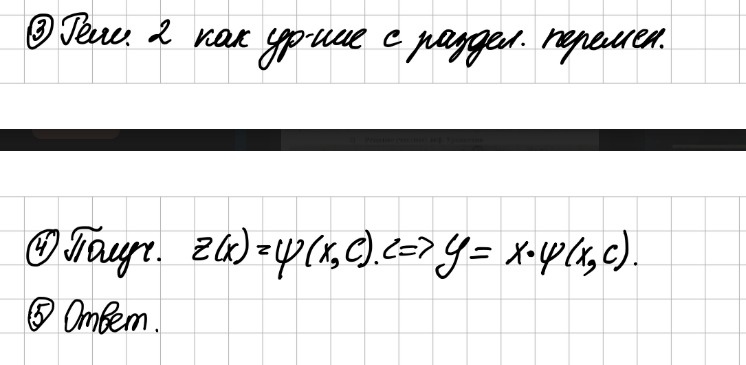
\includegraphics[width=0.25\linewidth]{Снимок экрана 2025-02-14 112453.png}
\end{figure}

 \subsection{Линейные дифференциальные уравнения первого порядка}

 ОПР: (1)



 \textbf{21.02.25}

 \textbf{Теорема 1} 

\section{Метод вариации производьной постоянной}

$y'+p(x)y=y(x)$

\textbf{Теорема}
Общее решение $y=e^(Sp(x)ex)$ $(Se^(Sp(x)cx)*q(xdx+c))$

Iэт. Решение соотв. однородное уравнение

$Y'+P(X)Y=0$, с разд, перем



ПРИМЕЧАНИЕ!Уравниния решаются только методом варианции

\subsection{Дефференцальные уравнения полных дефференцалах}

Опр: Рассмотрим дифф.ур-ие
$M(x,y)dx+N(x,y)dy=0$ - 1

Уравнение 1 назывется Уравнением в полных дифф-лах, если 

$\frac{\vartheta M(x,y)}{\vartheta y} \equiv \frac{\vartheta N(x,y)}{\vartheta x}$

Считаем что y=y(x), $ N(x,y) \neq 0 $
Тогда получаем по опр (1) эквив. уравнению
(3) $\frac{dy}{dx} = - \frac{M(x,y)}{N(x,y)}$

Алгоритм решения 

1 Пусть выполняется (2)

2 Найдем вспомогательную функцию $\Phi(x,y)$
как решение след. системы уравнения

\begin{figure}[H]
    \centering
    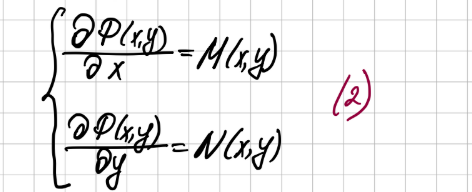
\includegraphics[width=0.25\linewidth]{Снимок экрана 2025-02-21 103834.png}
\end{figure}

3 Рассмотрим 1-е Уравнение в(*) решаем y. 
Тогда получем $\frac{d \Phi(x,y)}{dx} = M(x,y)$

$\Phi(x,y) = \int M(x,y)dx = \int_x0 x$ (винзу x0 и x сверху)
тут надо дополнить

4 Подставялем эту

5 Решим уравнение (отн.y)
(**) 

6


\textbf{Теорема 2}

Обноснования алгоритма

.....


Рассмотрим уравнение в симметрической форме

Уравнением в дифференциалах называется
уравнение

(1) A(x, y) dx + B(x, y) dy = 0,

$\frac{\vartheta A}{\vartheta y} \neq \frac{\vartheta B}{\vartheta x} $

(1) Не явяелтся ур-ием полных дефференцалов

\textbf{Теорема} Сущ-ие ф-ия $\mu(x,y)\neq 0$,т, 
(2) $\mu(x,y)   $

...



Опр: Функция $\mu(x,y)$ интегрируевым множитилем для ур(1)

Пример:




\textbf{Основаная теорема и единсвтенности}





\textbf{28.02.25}

\textbf{Оснвовная теорема Коши}
Если f(x,y) $\frac{\vartheta f (x,y)}{\vartheta y}$ - непр,

то задача Коши (1 -2) имеет единтсвенное решение

Док-во: I этап. Сведение 1 - 2 кинт уравнению 

(3) y(x)$y_0 +\int_{x_0}^{x}f(t,y(t))dt$

Мы доказали, что

1 - 2 $\Leftrightarrow $ (3) (их решенеия совп)

II этап. Решение (3)

Строится последовательность функции

$\varphi_0(x) = y_0, \varphi_1(x) = y_0 + \int_{x_0}^{x} f(t, \varphi_0(t))dt$

$\varphi_2(x) = y_0 + \int_{x_0}^{x} f(t, \varphi_0(t))dt$

(*) $\varphi_{n+1}(x) = y_o + \int_{x0}^{x} f(t,\varphi_n(t))dt$

Получем последовательность непрерывной функции

$\varphi_0(x), \varphi_1()x, \varphi_n(x)$


\begin{figure}[H]
    \centering
    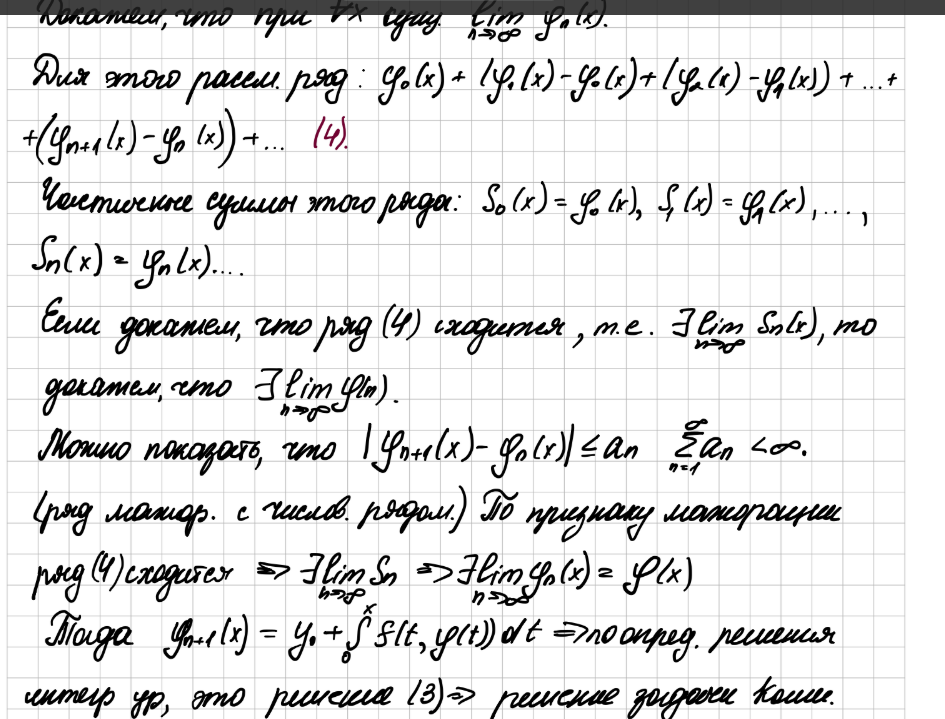
\includegraphics[width=1\linewidth]{Снимок экрана 2025-02-28 102203.png}
\end{figure}


III этап. Единсвтенность решения

Имеем $\varphi(x)$ реш (3)
Пусть $\varphi_1(x)$ точка решения (3)
т.е 

$\varphi(x) \equiv y_0 + \int_{x_0}^{x}f(t,\varphi(t)dt)$

$\varphi_1(x) \equiv y_0 + \int_{x_0}^{x}f(t,\varphi_1(t)dt)$

(4) $\varphi(x) - \varphi_1(x) \equiv \int_{x_0}^{x} \left[f(t,\varphi(t)) - f(t,\varphi)\right]dt$







\textbf{Теорема о среднем}
Если g(x) - диф. функ,
то $g(x_1) - g(x) = g'(\varepsilon )(x_1-x_1)$

$\varepsilon$ каждая точка между
Из (4)



...

...
...

\section{2 Раздел. Линейные дифференциальные уравнения n-го порядка}

Опр: Линейное обыкновенное дифференциальное уравнение n-го порядка
$a_0(x)y^{(n)}+a_1(x)y^{(n-1)} + ... a_n (x)y = f(x), a\leq x\leq b, y=y(x) - $ низв.

$a_0(x),a_1(x),...a_n(x)$ заданные непр функции



Опр: Линейнре уравнение назывется однорондным, если $f(x) \equiv 0,$,
Линейнре уравнение назывется неоднорондным, если $f(x) \neq  0,$

Опр: Функция $\varphi(x)$ нызвается решением (частный) уравнения (1), если 

$a_0(x)y^n(x)+...+a_n(x)y(x) = f(x)  $ .

Решение:

Короче надо будет запонлнить пробелы тут


\textbf{07.03.25}

Опр: Линейно зависимые и линейно независимое функции 
$\varphi_1(x),... \varphi_m(x)$ на $[a,b]$

\begin{figure}[H]
    \centering
    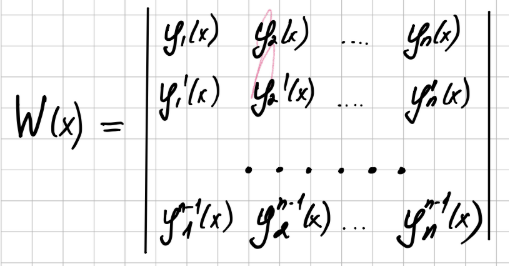
\includegraphics[width=0.25\linewidth]{Снимок экрана 2025-03-07 100524.png}
\end{figure}

\textbf{Теорема 2} Если $\varphi_1(x),... \varphi_m$ - линейно зависима на 
$[a,b]$, то W(x)=0

Доказательство: Пусть $\varphi_1(x),... \varphi_m(x)$ линейно зависимана 
на $[a,b]$ $\exists\alpha_1,...,\alpha_m$ не всеравно Об т.ч

$\alpha_1, \varphi_1(x)+,...,\alpha_m, \varphi_m(x) \equiv 0 \Leftrightarrow \alpha_i=0 \bar{i=1,m}$


\begin{figure}[H]
    \centering
    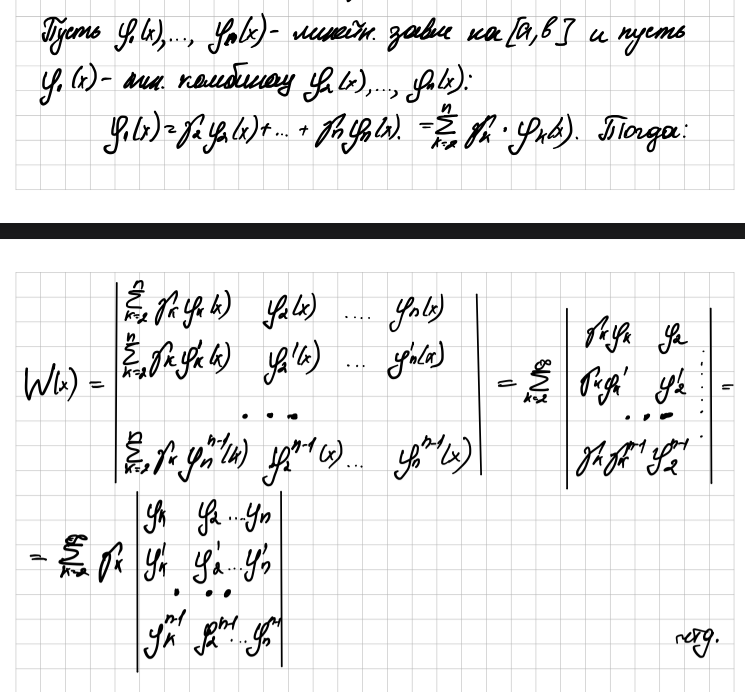
\includegraphics[width=0.25\linewidth]{Снимок экрана 2025-03-07 102029.png}
\end{figure}



Рассмотрим линейное однородное уравнение
$(1) y^{(n)}+a_1(x)y^{(n-1)}+,...,a_n(x)y=0,$ или $l(y) = 0 a\leq x \leq b $

Доказательство: Предположим противное : $\exists x_0 \in [a,b] W(x_0)=0$
По теории из алгберы столбцы определителя $W(x_0)$ линейно зависимы:
$\exists \alpha_1,..\alpha_n$ числа не все 0, такие что 


\begin{figure}[H]
    \centering
    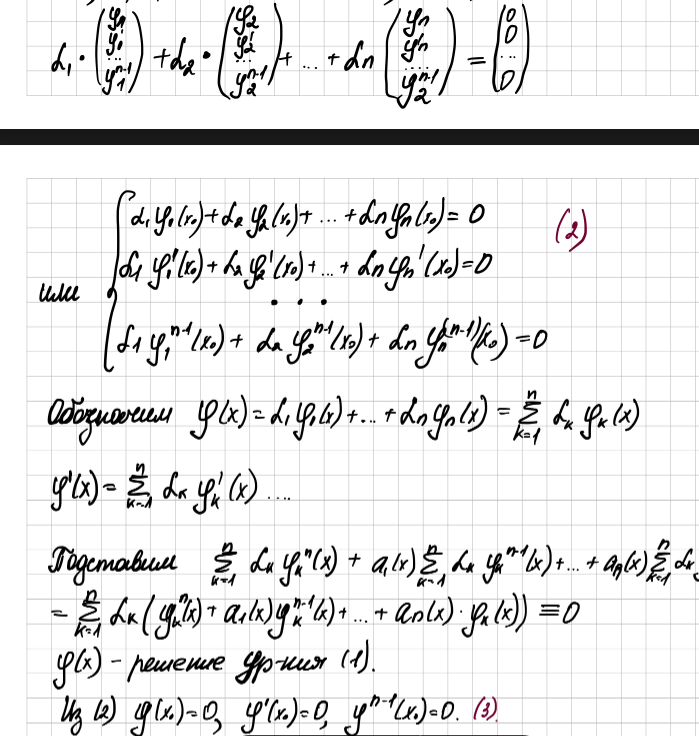
\includegraphics[width=0.25\linewidth]{Снимок экрана 2025-03-07 103059.png}
\end{figure}

\begin{figure}[H]
    \centering
    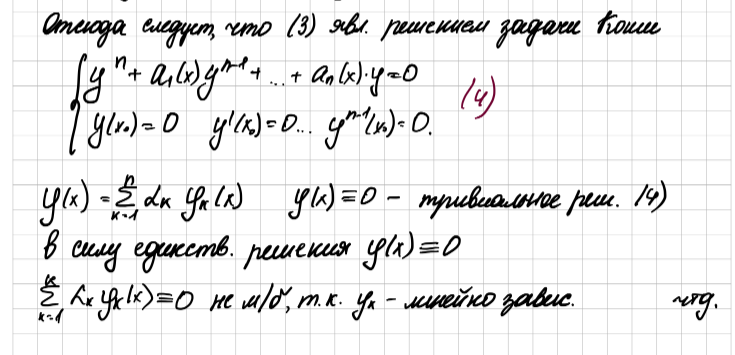
\includegraphics[width=0.25\linewidth]{Снимок экрана 2025-03-07 103128.png}
\end{figure}


Отступление 

\begin{figure}[H]
    \centering
    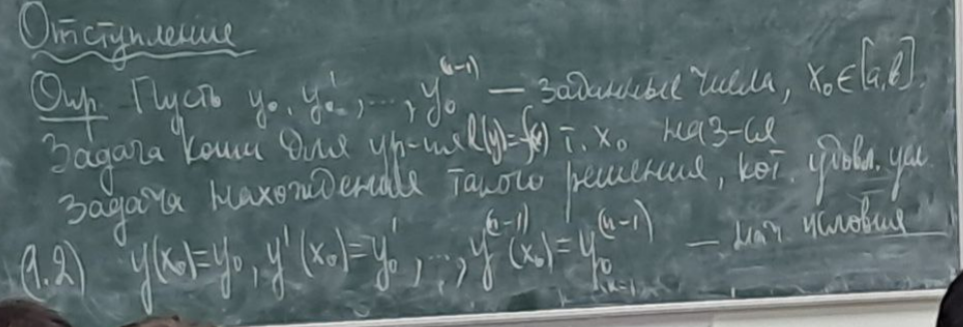
\includegraphics[width=1\linewidth]{Снимок экрана 2025-03-07 103827.png}
\end{figure}


\textbf{Теорема} о существовании решенеия задачи Коши для линейного уравнения

Имеет единтсвенное решения для линейного уравнения имеет единтсвенное решение
$\forall x_0 \in [a,b], y_0, y_0',...$


Конец отступления


Тут нужно везде заполнить пробелы, в крайнем случае попросить людей которые лучше конспектировали лекцию


\textbf{Теорема 4}




\textbf{14.03.25}


\textbf{Теорема 6}


Обоснования метода варианции

\end{document}